%!TEX root = ../thesis.tex
% ******************************* Thesis Appendix B ****************************

\chapter{Minimum DC Gain of an OTA in an Incremental-\(\Delta\Sigma \)}
\label{app:integrator-inl}

This section investigates the impact of the DC Gain of an OTA inside the SC-Integrator on the first stage of the proposed architecture: an Incremental-\(\Delta\Sigma \).

The assumption made is a unity gain frequency of the OTA is such wide that the error on the settling of the integrator is only due to the OTA DC Gain.

Moreover, process mismatch is disregarded and the passive-adder with comparators are supposed to be ideal.

\begin{figure}[htp]
    \centering
    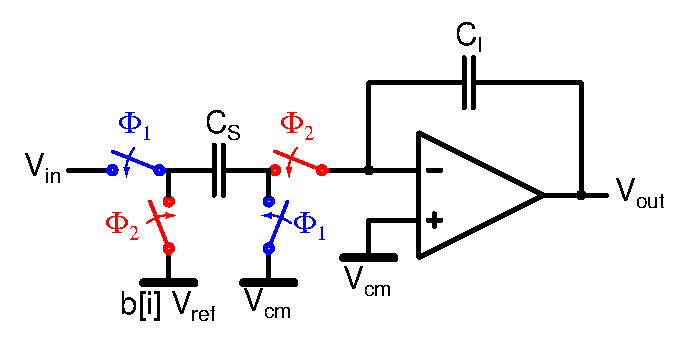
\includegraphics[width=0.7\textwidth]{Appendix2/sc-integrator.ps}
    \caption{Two-Phase SC Integrator implemented}
    \label{fig:app-sc-integrator}
\end{figure}

In such circumstances the SC-Integrator of the \figurename~\ref{fig:app-sc-integrator} respects the equation~(\ref{eqn:app-sc-integrator}) where A is the OTA DC Gain, \(C_S \) the sampling capacitor, and \(C_I \) the integration capacitor.

\begin{equation}
    \label{eqn:app-sc-integrator}
    V_{out}[n] = V_{out}[n-1] \left(\frac{1+\frac{1}{A}}{1+\frac{1+C_S/C_I}{A}}\right) + (V_{in}-b[n-1]V_{ref})\frac{C_S}{C_I}\left(\frac{1}{1+\frac{1+C_S/C_I}{A}}\right)
\end{equation}

One could note the ratio of \(C_S/C_I \) deeply impact the error at each integration step. In order to decrease the DC Gain requirement is to reduce this ratio to the maximum. Therefore a ratio of 1 is a good candidate.

By recurrence, the residue of this stage being the output of the integrator, the residue can be expressed as

\begin{equation}
    V_{out}[n] = V_{out}[0] {\left(\frac{1+\frac{1}{A}}{1+\frac{1+C_S/C_I}{A}}\right)}^n + \frac{C_S}{C_I}\frac{1}{1+\frac{1+C_S/C_I}{A}}\sum_{i=1}^{n} {(V_{in}-b[n-1]V_{ref}) {\left(\frac{1+\frac{1}{A}}{1+\frac{1+C_S/C_I}{A}}\right)}^i}
\end{equation}

The incremental mode resetting at each new sample, the initial output value is zero. Therefore, the residue only depends on the transfer of charges from the sampling to the integration capacitor. The maximum of error is governed by the threshold voltage of the 1.5-bits quantizer following our architecture.

The error committed by a finite gain is thus
\begin{equation}
    V_{error}[n] = \frac{C_S}{C_I}\sum_{i=1}^{n} {(V_{in}-b[n-1]V_{ref}) \left[\left(\frac{{\left(1+\frac{1}{A}\right)}^i}{{\left(1+\frac{1+C_S/C_I}{A}\right)}^{i+1}}\right)} - 1\right]
\end{equation}

To consider the ADC does not need calibration, we could assume that the error is below half LSB of the desired accuracy. In this case, the residue displays the maximum of the error at the transition between two adjacent codes. As the input range is \(2 V_{ref} \), a transition for a 1.5-bit quantizer whose threshold voltage are \(\pm V_{ref}/2\) occurs at \(V_{ref}/(2\times OSR) (1+2k) \) where \(k \) is a signed integer.

\begin{equation}
    \frac{V_{error}[n]}{V_{LSB}} = 2^{NBits} \frac{C_S}{C_I} \left(
    \frac{1}{4 OSR} {\left[\sum_{i=1}^{n}\left(\frac{{\left(1+\frac{1}{A}\right)}^i}{{\left(1+\frac{1+C_S/C_I}{A}\right)}^{i+1}}\right)}\right] - N \right)
\end{equation}


We could also assume this this equivalent to say the integral non linearity fits into the bounds for the desired accuracy. INL error is described as the deviation, in LSB or percent of full-scale range (FSR), of an actual transfer function from a straight line. The INL-error magnitude then depends directly on the position chosen for this straight line. At least two definitions are common: `best straight-line INL' and `end-point INL'.

\textbf{Best straight-line INL} provides information about offset (intercept) and gain (slope) error, plus the position of the transfer function (discussed below). It determines, in the form of a straight line, the closest approximation to the ADC's actual transfer function. The exact position of the line is not clearly defined, but this approach yields the best repeatability, and it serves as a true representation of linearity.

\textbf{End-point INL} passes the straight line through endpoints of the converter's transfer function, thereby defining a precise position for the line. Thus, the straight line for an N-bit ADC is defined by its zero (all zeros) and its full-scale (all ones) outputs.
The best straight-line approach is generally preferred, because it produces better results. The INL specification is measured after both static offset and gain errors have been nullified, and can be described as follows:

Let consider the case of the maximum error compared to a straight line passing by end-points of the transfer function:
\begin{equation}
    INL = \max \left| V_{out}(code)-V_{out}(code_{\min}) - (code-code_{\min}) \times slope  \right|
\end{equation}

where the slope is 
\begin{equation}
    slope = \frac{V_{out}(code_{\max})-V_{out}(code_{\min})}{code_{\max}-code_{\min}}
\end{equation}

For the sake of clarity, let us normalize voltages and codes between 0 and 1. As in a first order Incremental-\(\Delta\Sigma \) the estimation is the average of output bits the normalized estimation of the output code is given to be \(ec = \frac{1}{OSR}\sum_{i=1}^{OSR} b[i] \). 

We deduce that the output estimation is the sum of $ec$ and the residue weighted by \(1/(2 OSR)\).  Considering \(V_{out}(1) \) and \(V_{out}(0) \) at a transition between two `extra' codes, they are respectively given by \(1-V_{error\max}[n] \) and \(V_{error\max}[n] \).

the INL being
\begin{equation}
    INL = \max \left| V_{out}(ec)-V_{out}(0) - ec (V_{out}(1)-V_{out}(0))  \right|
\end{equation}

and replacing \(V_{out}(1) \) and \(V_{out}(0)\) by their value leads to
\begin{equation}
    INL = \max \left| ec + V_{error\max } [n] + V_{error}[n, ec] - ec (1 - 2 V_{error\max }[n])  \right|
\end{equation}

which admits a maximum of \(4 V_{error\max }[n] \)

Therefore, to prevent a calibration with respect to the INL, the DC gain constraint on the OTA is increased by 2-bits.
